\documentclass{article}
% setup page
\usepackage[utf8]{inputenc}
\usepackage{fancyhdr}
\usepackage[a4paper, top=2.5cm, left=2cm, right=2cm, bottom=2cm]{geometry}
\usepackage{titling}

% for random text
\usepackage{lipsum}

\usepackage{todonotes}

\usepackage{amsmath}
\usepackage{graphics}
\usepackage{multirow}

\usepackage[backend=biber]{biblatex}
\addbibresource{papers.bib}


\DeclareSourcemap{
  \maps[datatype=bibtex]{
    \map[overwrite=true]{
      \step[fieldset=urldate, null]
      \step[fieldset=url, null]
      \step[fieldset=note, null]
    }
  }
}

% setup info
\title{IR Project 1: Report}
\author{Tobias Veto, Philip Junker, Marc Fischer}

% setup header/footer
\pagestyle{fancy}
\fancyhf{}
\rhead{\theauthor}
\lhead{\thetitle}
\rfoot{Page \thepage}
 

\begin{document}

\section*{TODO}
\begin{itemize}
	\item result files
	\item readme file
	\item package code and results
	\item finish report
\end{itemize}

 
\section*{Introduction}
For the implementations of the naive bayes, logistic regression and SVM we stayed close to the code shown in the lecture. Thus the implementations of the algorithms were straightforward while optimization and data preprocessing were challenging. Most of our effort went into the data pruning.

In our team one person each focuses on one classifier. While we shared insights, and the code that we use for the reader, this might account for inconsistencies in the code and different tone in the chapters of this report.


\section*{Data transformation and pruning}
A big part of our implementation was data preprocessing. We read the tokens from the documents (with tinyIR), remove tokens not consisting of letters, stem the word and remove stopwords. \cite{joachims_text_1998,ozgur_text_2005} both list this as the standard approach to preprocessing in document classification. From the resulting corpus of documents we remove those that occur less then \texttt{minOccurrence} and those that are found in more than $\text{\texttt{maxOccurrenceRate}} \cdot \text{\texttt{nrDocuments}}$, where $\text{\texttt{maxOccurrenceRate}} \in (0, 1]$.
The resulting dictionary of words is uses to rerpresent each document as a bag-of-words vector. For the weights within the vector we use boolean weights (1 if the word occurs in the document, else 0), tf-idf weights (inspired by \cite{ozgur_text_2005}) and the count of word.  \todo{specify weighting method here} has generally yielded the best result.
We also discovered, that words extracted from the title of the document contain a high amount of information and lend themselves especially to predicting country codes. The words from the titles were processed like the words from the content.

We also tied to access the data in a random order. Our assumption was that some classes might only show up at the end of the stream of documents and thus, might only be encountered with a very low learning rate (in Logistic Regression and SVM).
However, the random order had only negligible effects on the performance of the algorithms. As the order is irrelevant for the Naive Bayes approach, this has no impact on it.

\section*{Naive Bayes}
We used the formulas for Naive Bayes as shown in the lecture. For each code we calculated the probability $P(word | code)$ for every word in the reduced dictionary.
For each of the three different code-types a different threshold was evaluated. The advantage of this approach is the independence of the code-types and therefore the possibility of a country-code to be predicted although the probability for this code given a document is much lower than for all the topic-codes. The performance in form of F1-scores is plotted for both country- and topic-codes in figure \ref{fig_bayesThreshold}. Because the industry-codes are very hard to predict the optimal threshold for these codes turned out to be zero, meaning we do never predict an industry code.
While the word-code-probabilities for the topic-codes were calculated using the content of the Reuters-articles we used only the article-titles to calculate the probabilities for the country-codes. 

The training of the model needs constantly 1.3GB of RAM. The training of the topic-codes took around 160 minutes in total to train the topic-codes (80 minutes) and the country-codes (80 minutes). The training was done on a laptop with an intel i7 (2.9GHz) with 8GB of RAM.

\begin{figure}[h!]
    \centering
    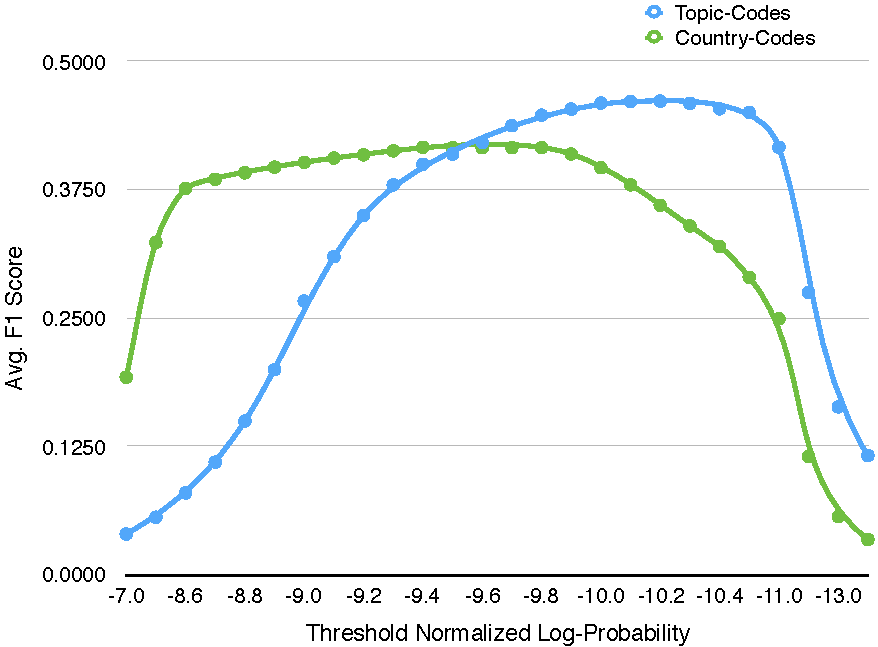
\includegraphics[scale=0.6]{graphics/BayesF1ScoreTopicCountry.pdf}
    \caption{This figure shows the average F1-Score of topic- and country-codes using different thresholds for the normalized log-probability.}
    \label{fig_bayesThreshold}
\end{figure}

\section*{Logistic Regression}
\subsection{Label Types}
        We quickly saw that the problems of predicting the different label types were very different. For example there were usually more topic codes than  country codes per document. Furthermore, the industry codes were usually much harder to predict as they were structured in a hierarchical manner and there were more of them overall. Therefore we treated each label type independently, and applied variants of our general approach:
            \subsubsection{ Topic codes}
                This was the part where we had the least problems. the cutoffFinder lead to best results.  We reached a F1-score of around 0.35 on topic codes.

            \subsubsection{ Country codes }
                Here using the same approach as for topic codes worked fine, leading to a F1-score of around 0.20. However, we found out that using the document titles instead of the content lead to better results, since the name of the country of the interest was often present in the title. A second variation of the general approach we used was to manually determine the cutoff. The intuitive approach of targeting the same average of labels assigned (using the cutoffFinder) lead to some (especially longer) documents having a lot of country codes assigned, and some having none.
                    Combining these two adjustments lead to a F1-score of around 44 for country codes.


            \subsubsection{industry codes }
            Predicting the industry codes with our current approach was very hard. There were many more industry codes than any other codes, and some of the industry codes were very rarely assigned.  Combined with the fact that our algorithm proceeded in an online manner, weighting some documents more than others, it was very hard to reach a F1-score higher than 0.10 (when focusing solely on industry codes). However, we observed that most of the time, there was no industry label to predict. Since predicting one when there was in fact none had a negative effect on the precision of our prediction, we chose the strategy to never predict any topic codes.

            Combining the three different predictors into one, we got a F1-score of around 0.4

    \subsection{Processing time and memory footprint}
        Our alogrithm required approximately 1.9 GB of memory and took around 12 minutes to compute.

\section*{SVM}
The algorithm shown in the lecture is the well-known pegsasos algorithm\cite{shalev-shwartz_pegasos:_2011,shalev-shwartz_pegasos:_????}. For the implementation we train one SVM per category occurring in the training data in an all-vs-one approach.
Table~\ref{table:svmResults} shows the results of various approaches.
Data was preprocessed as introduced before with the use of homogeneous coordinates (bias term) and without. The listed papers suggest, not using a bias with the normal formulation of the pegasos algorithm or to adjust it if doing so, as it undermines the convergences guarantee. As the bias them is just a very small change (second decimal place) and was thus omitted. For the parameter $\lambda$ the optimal choice seems to be around $10^{-4} - 10^{5}$. Seems consistent when changing other parameter of the algorithm. Thus further tests were only run with those lambdas.

Reducing the dictionary size helped to increase performance and slightly increase the score. So the final version (bold) uses only tokens extracted from titles, but all of them.

\begin{table}[h]
\centering
\resizebox{\textwidth}{!}{
	\begin{tabular}{|l|l|l|l|l|r|r|r|r|r|}
	\hline
	$\lambda$ & \texttt{minOccurrence} & \texttt{maxOccurrenceRate} & Dictionary,Weights & Resulting \# Words & Run Time & Memory Consumption & Avg. Precission & Avg. Recall & Avg. F1-Score\\
	\hline
	1 & 1 & 0.2 & tokens, count-weights & TODO & 123 min & 8 GB & 0.295 & 0.053 & 0.08\\ \hline
	1 & 3 & 0.2 & tokens, count-weights & 39249 & 28 min & 3.4 GB & 0.30 & 0.053 & 0.09\\ \hline
	0.1 & 3 & 0.2 & tokens, count-weights & 39249 & 28 min & 3.7 GB & 0.30 & 0.053 & 0.09\\ \hline
	0.01 & 3 & 0.2 & tokens, count-weights & 39249 & 19 min & 3.4 GB & 0.55 & 0.11 & 0.19\\ \hline
	0.001 & 3 & 0.2 & tokens, count-weights & 39249 & 15 min & 3.5 GB & 0.88 & 0.19 & 0.31\\ \hline
	0.0001 & 3 & 0.2 & tokens, count-weights & 39249 & 14 min & 3.4 GB & 0.92 & 0.20 & 0.33\\ \hline
	0.00001 & 3 & 0.2 & tokens, count-weights & 39249 & 14 min & 3.4GB & 0.92 & 0.20 & 0.33\\ \hline
	0.0001 & 10 & 0.2 & tokens, count-weights & TODO & 7 min & 3 GB & 0.92 & 0.20 & 0.33\\ \hline
	0.0001 & 20 & 0.2 & tokens, count-weights & TODO & 5 min & TODO & 0.92 & 0.20 & 0.33\\ \hline
	0.0001 & 20 & 1 & tokens, count-weights & TODO & 5 min & 3.1 GB & 0.92 & 0.20 & 0.33\\ \hline
	0.0001 & 0 & 1 & titles, count-weights & 22871 & 8 min & 3.1 GB & 0.93 & 0.21 & 0.34\\ \hline
	\textbf{0.0001} & \textbf{0} & \textbf{1} & \textbf{titles, boolean weights} & \textbf{22871} & \textbf{8 min} & \textbf{3.1 GB} & \textbf{0.94} & \textbf{0.21} & \textbf{0.34}\\ \hline
	0.0001 & 0 & 1 & titles, tf-idf weights & 22871 & 8 min & 3.1 GB & 0.90 & 0.20 & 0.32\\ \hline

	\end{tabular}
}
\caption{Test Results for the SVM. All tests were done on a Machine with 32 GB ram and a high java heap size, thus java never deallocates memory. On another machine with less memory the memory consuption of the SVM code s only around 2 GB for most cases. The bold line shows what is used for submission and what is the current default.}
\label{table:svmResults}
\end{table}

The SVM achieves very high prcesision, but poor recall indincating that it is too strict (not giving labels that should be there). Lowering the $\lambda$ parameter could solve this, but does not do so on in this case. This might indicate a non-linearly sperable set. This would suggest the usage of kernels. The results from \cite{joachims_text_1998} strongly suggest that polynomial or RBF kernel work well. However due to performance considerations we did not consider this in the first place and did not revisit it later due to time constraints.

\printbibliography

\end{document}